\section{Experimental Setup}
To evaluate the effectiveness of our symmetry elimination technique we performed
a comparative analysis using A* on a number of benchmarks taken from
the freely available pathfinding library 
Hierarchical Open Graph (HOG)\footnote{\url{http://www.googlecode.com/p/hog2}}:
\begin{itemize}
\item{\textbf{Adaptive Depth} is a set of 12 maps of size 100$\times$100 in which approximately
$\frac{1}{3}$ of each map is divided into adjacent rectangular rooms of
varying size and the rest of the map is a large open area interspersed with 
large randomly placed obstacles.}
\item{\textbf{Baldur's Gate} is a set of 120 maps taken from BioWare's popular
roleplaying game \emph{Baldur's Gate II: Shadows of Amn}. 
Often appearing as a standard benchmark in the literature 
\cite{botea04,bjornsson05,bjornsson06,sturtevant05,harabor08} these maps range in 
size from 50$\times$50 to 320$\times$320 and have a distinctive 45-degree orientation.}
\item{\textbf{Rooms} is a set of 300 maps of size 256$\times$256 which are divided into 32$\times$32
rectangular areas that are connected by randomly placed entrances.}
\end{itemize}

% \begin{figure}[t]
%        \begin{center}
%                        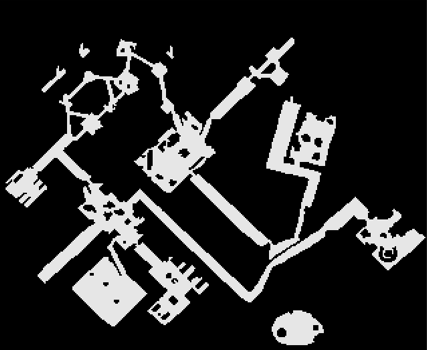
\includegraphics[width=0.6\columnwidth, trim = 10mm 10mm 10mm 0mm]{diagrams/bgmap.png}
%        \end{center}
%        \caption{A map from BioWare's \emph{Baldur's Gate II}}
%        \label{fig-bgmap}
% \end{figure}
%\par
Since our work is applicable to both 4 and 8 connected grid maps we used two
copies each map: one in which diagonal transitions are allowed and another
in which they are not.
For each map we generated 100 valid problem instances, checking that every
instance could be solved both with and without the use of diagonal
transitions.
We then ran A* twice: once on the original (4 and 8 connected) maps and again 
on our modified (4 and 8 connected) maps. 
This makes for a total of 172800 (864$\times$100$\times$2) distinct experiments.
Our test machine had a 2.93GHz Intel Core 2 Duo processor, 4GB RAM and
ran OSX 10.6.2.
We use the A* implementation provided in HOG.
